\documentclass[a4paper,11pt]{article}
\usepackage[utf8]{inputenc}
\usepackage{graphicx}       % front image
\usepackage{hyperref}       % links and email
\usepackage[english]{babel} % linebreaks for english words
\usepackage{eurosym}
\usepackage{listings}
\usepackage{amsmath}
\usepackage{tfrupee}

%Can Also be used for Location of high importants like Parliament and Embassies

% opening
\title{{Advanced Threat Detection \& Tracking at Locations of High Value using Cutting Edge Modern Digital Solutions}}
\author{Animesh Renanse}

\begin{document}

\begin{titlepage}
    \centering
    \maketitle
    \thispagestyle{empty}   % discard page number
    \includegraphics[width=2cm]{logo.png}
    \vfill
    {\raggedright
    Animesh Renanse\\
    IIT Guwahati\\
    \href{mailto:animesh.r18a@gmail.com}{animesh.r18a@gmail.com}\\
    \textit{All Diagrams were made in open source package Inkspace}\\
    }
\end{titlepage}

\begin{abstract}
\section{\textbf{Preface}}
\subsection{Objective} 
\textit{Objective of this proposal is to Provide an Efficient System cum Methodology to Improve Security and Threat Detection at Airports, Embassies, Parliament and other Places of High Value and Importance using AI \& other Modern Approaches.}
\newline

\subsection{Overview}
In the forthcoming sections, I will explain how this proposal, \textbf{while involving JSW group's resources}, can drastically increase the security at some of the most vulnerable locus of the contemporary modern world, i.e Airports, Parliament and other Place of High Value, using recent technical advances in the field of Neural Networks, A.I. \& IoT in general which has enabled faster than ever communication between different \textit{Intelligent Systems} to determine Threat \& qucikly raise it up to the concerned Security Elements.
\newline\newline
This Proposal, thus, tries to counteract one of the major \textit{Socio-Economic} Problem India is facing currently, which is no other than \textbf{Terrorism}, which in the face of recent tensions in the vicinty of our borders have engrained a sense of fear in the populus of India, which can only be made sure doesn't become a reality if we strengthen our Security Systems \& Quick Reaction Elements so that even in the face of such crisis, due to our apprehension, we act quickly and eliminate the threat before it concludes it's intentions.
\newline\newline
The motivation for this proposal was engrained due to ceaseless breaches in our Security System from time to time which was either due to irreplaceable laxity of humans who performed the job or the lack of clarity in the order and direction systems, which, with much sorrow, \textbf{led to the \textit{2001 Parliament Attacks}} and countless other small attacks and breaches in other governmental and public spaces.\newline\newline
This provided nothing but motivation for developing a new Security System, which addresses the redundant behavior of human workforce by introducing \textit{Cutting Edge Modern Approaches} which includes Artificial Intelligence and their synchronization with other hardware, which in a whole is Internet of Things.

 \vfill
    {\raggedright
    \textit{All Diagrams were developed in an open source package called Inkspace}\\
    }
%Write motivation in "Overview"

%LEVELS OF THREAT
%gamma_1 phase, human input
%gamma_2 phase, human input
%worst case scenario analysis









%TODO::Who: Who will do the work, who will manage the work, and who does the customer call if there is a problem?
%What: What needs to be done or delivered, what will be required to do it, what can the customer expect, and what will it cost them?
%Where: Where will the work be done, and where will it be delivered?
%When: When will you start, when will key milestones be scheduled, when will the project be complete, and when is payment due?
%How: How will work be done, how will it be deployed, how will it be managed, how will you achieve quality assurance and customer satisfaction, how will risks be mitigated, how long will it take, and how will the work benefit the customer?
%Why: Why have you chosen the approaches and alternatives you have selected, and why should the customer select you?
\end{abstract}
%\setcounter{section}{0}
\newpage
\tableofcontents
\pagebreak
\section{Executive Summary}
\begin{itemize}
\item{This proposal, If applied to various Locations of higher Importance will ensure that the security of such locations is never compromised.}
\item{Even in the \textit{drop-dead} extreme case, it will ensure that the Reaction by the Security Units is \textit{fast} as well as \textit{organized}, which will ensure that the Threat is always kept tracked of.}
\item{The Whole System is divided in two phases, one is \textit{Primary Phase (will be called $\gamma_1$) } which will do a preliminary scan of the threat by the System combined with the human input in the form of security personnel at the checkpoint.}
\item{The other phase is called \textit{Secondary Phase (will be called $\gamma_2$)} present inside the perimeter of the location, which will receive, if there is any, level of threat from Primary Phase which will keep track of the threat, unless reset by the main security personnel in the perimeter.}
\item{Thus, in-case of any mishap, the security team will be aware of the position of possible threat and thus can neutralize the same with ease.}
\item{This proposal can easily be integrated with the already in process of being automated support systems at the Airports which uses Biometric Recognition of individual passenger for better service through A.I. to fully utilize the extent of A.I. that we can avail, which will stretch from Security Systems, which this proposal covered to the already being implemented support systems for Quality Service at Airports and other Locations of mass Gathering \textbf{\cite{AI Already}}}
\item{Since this proposal is on Improvement of current Security Systems, which include Cutting Edge Digital solutions, thus will require a bit high monetary resources, which, if followed the Equipments and services mentioned in the references will cost around \rupee8,81,000 \textbf{which is almost on par with the current manual security systems that is currently in service, not to mention it automates various tedious tasks like \textit{Threat Tracking and Detection}, which improves security by many folds.}}
\item{Finally, this can serve as a base for even Advanced Security systems that may be introduced in future to work upon it \textbf{due to this proposal being Modular}}
%AnY ENTRY SHOULD BE ABOVE THE LAST ITEM GIVEN BELOW
\item[$\star$]{\textit{Please refer to References page to find out how and which different products for different tasks are \textit{proposed} to be used.}}
\end{itemize}
\section{Proposal Description}
\subsection{The Primary ($\gamma_1$) Phase}
 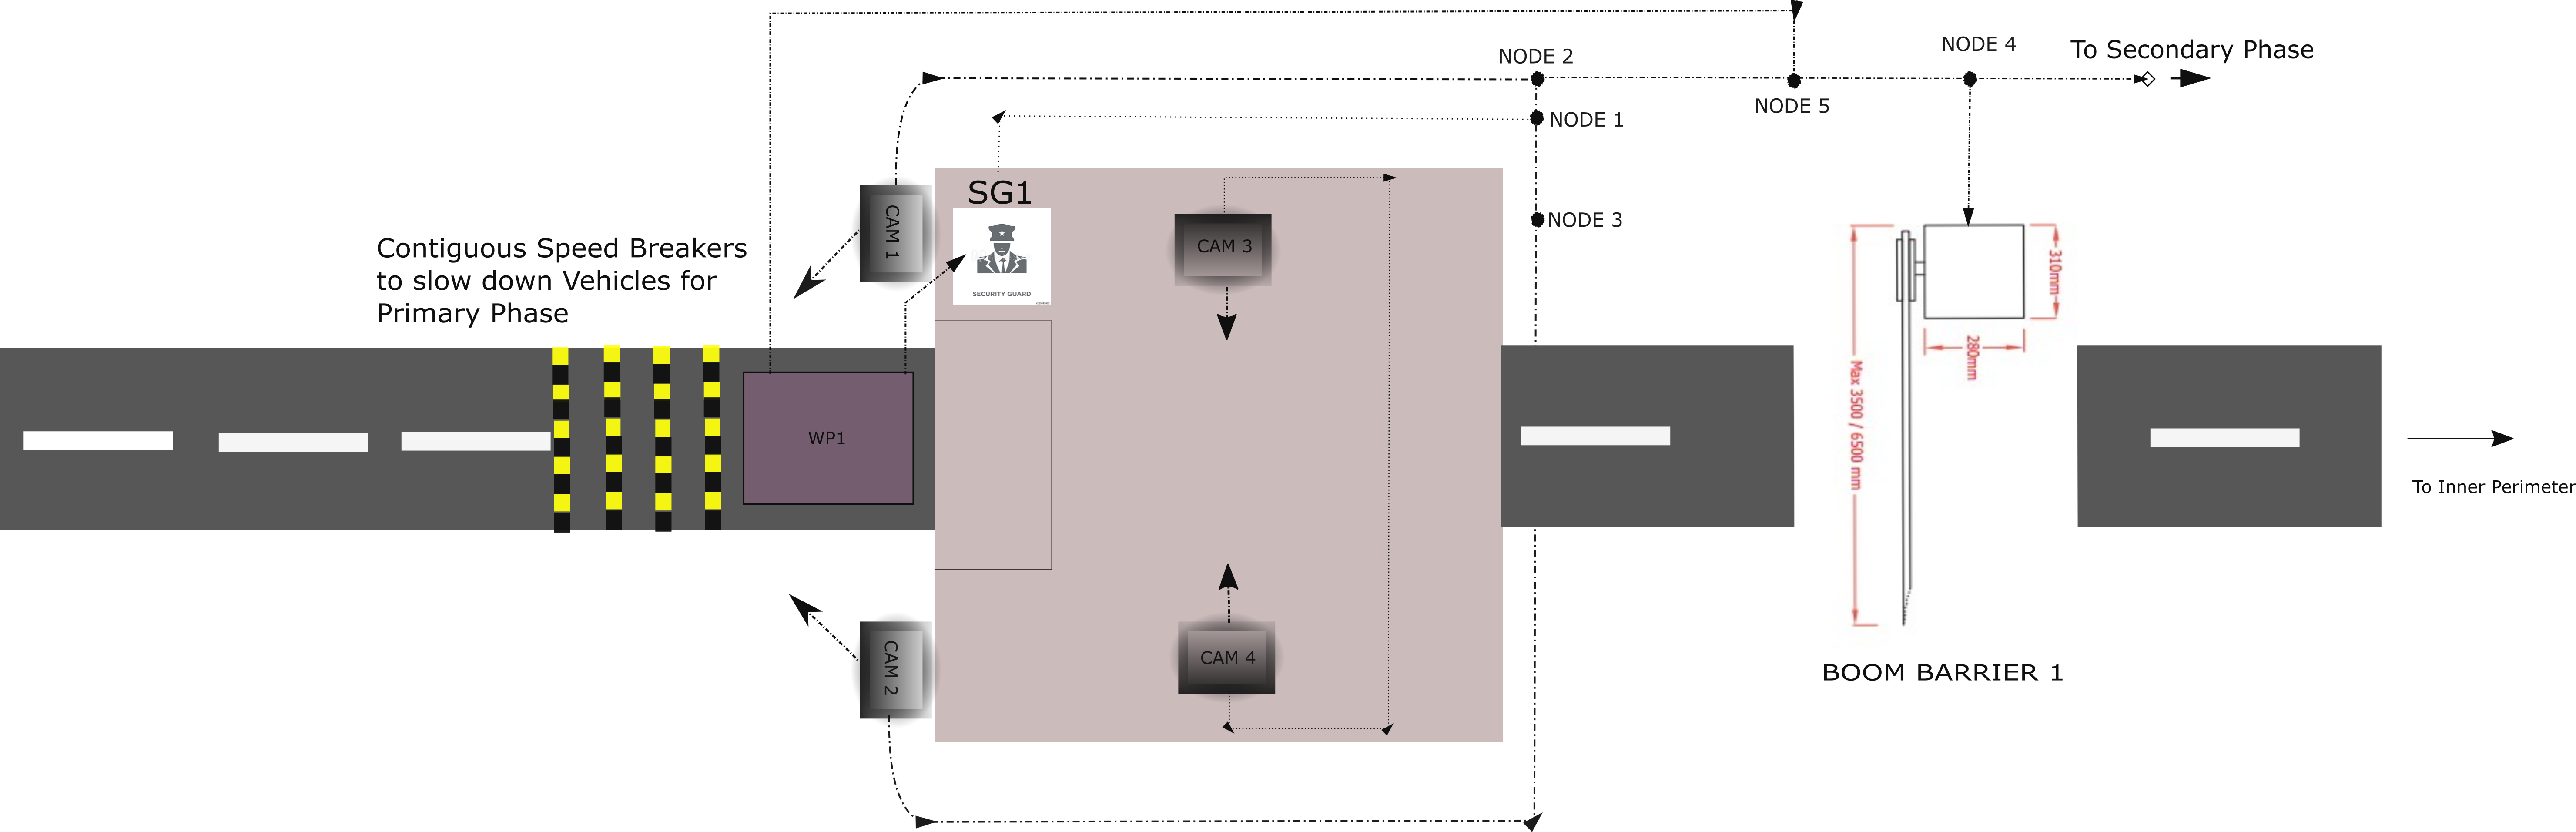
\includegraphics[width=8cm,height = 19cm ]{Primary Phase.png}
\subsubsection{In-Depth: The $\gamma_1$ Phase}
The $\gamma_1$ Phase is the first phase of the this proposal through which any sample will go through, it contains both machine and human inputs and both work in conjunction towards the final goal of giving a score of \textit{Threat Induced by the given sample} which is passed on to the $\gamma_2$ Phase, which will be discussed shortly.
\newline\newline
The various elements in the $\gamma_1$ Phase are as follow:
\begin{itemize}
\item{WP1: The Industrial Weighing platform \textbf{\cite{Weighing Platform}}, this will be used for weighing the incoming vehicle, this weight will be used for computing level of threat with the use of other inputs as well.}
\item{CAM 1 \& CAM 2: Two Industrial cameras, CAM 1 for for recognizing License Number of the car  \textbf{\cite{LP camera}} and CAM 2 for recognising Facial Condition of the driver and the side Passenger in the vehicle \textbf{\cite{FaceRecogCam}}, which is stored for only the time till the car is in $\gamma_1$ phase and is not of Immediate Threat (judged by the final score in $\gamma_1$ phase).}
\item{SG1: The Mandatory Security Personnel at the checkpoint, he will primarily be the human input in the pipeline who will give a score to the given sample's total Threat Score by choosing from a given set of threat level (explained soon) the personnel thinks best fit the given sample. The personnel also has access to the all the scores at all times especially the weight of the vehicle.}
\item{CAM 3 \& CAM 4: Two more industrial cameras \textbf{\cite{FaceRecogCam}} which will, in conjunction with CAM 2 will find out the total number of passengers in the vehicle.} 	
\item{NODE 1,2,3 \& 4: Node 1 is where the human input in the pipeline meets the other scores. Node 2 is where the scores from Node 1 (SG1) and Node 3 meet together and are aggregated and passed on to the next node. Node 3 is where the data from CAM 3 \& CAM 4 are converted to integer using Body/Face Detection \textbf{\cite{FaceFirst Platform}} which will compute the number of passengers and then will pass on to the next node. Node 4 is the the place where the numbers collected so far are computed, aggregated and worked upon to give a final score. Node 5 is the place where the weight of the vehicle comes to the picture, this weight is compared against the total passengers in the vehicle, if it is not under certain range, this will cause a negative loss towards the final score (\textit{Algorithm is given in the following subsection}) which is computed in Node 4.%Try to do something to get rid of various car weights itself%Please explain this whole passage in-depth and also how-to
}

\item{BOOM BARRIER 1: This Boom Barrier \textbf{\cite{Boom Barrier}} is supposed to be idle unless, the score of \textit{Threat is too high or the Security Personnel (SG1) deems another thorough check of the vehicle.}}
++++
\end{itemize}
After the completion of $\gamma_1$ Phase, we continue towards the $\gamma_2$ Phase which is inside the perimeter of the location which is being guarded.
\subsubsection{Algorithm to approximate the Luggage Weight}
In this section, the algorithm to approximate the weight of luggage of the car is introduced.\newline
After the vehicle goes through WP1, CAM 3 \& CAM 4, we have three sets of data:\newline
\begin{itemize}
\item{$W_F$ : Weight of front axle of the vehicle}
\item{$W_R$: Weight of rear axle of the vehicle}
\item{n : Total number of passengers in the vehicle, collected from CAM 3 \& 4}
\end{itemize} 
Now, some assumptions:-
\begin{itemize}
\item{Average weight of male: 80 kg, let the number of them detected be $n_1$}
\item{Average weight of female: 64 kg, let the number of them detected be $n_2$}
\item{Average weight of child $<$ 13 years: 35 kg, let the number of them detected be $n_3$}
\end{itemize}
Thus, the $W_{Pass} = n_1*80 + n_2*64 + n_3*35$\newline\newline
Now, After some calculation, we will get that \textit{Fraction of Load of vehicle on the front axle is given by:-}\newline\newline $\alpha = (1- \frac{W_F - W_R}{W_{Pass} + W_{Lugg}})/2$\newline
Due to lack of space, I'm skipping it's derivation.\newline\newline
By approximating $\alpha \approx 0.3584$, we can figure out $W_{Lugg}$ as:-\newline\newline
\boxed{W_{Lugg} = \frac{W_F - W_R}{1 - 2*0.3584} - W_{Pass}}\newline where, we know $W_F, W_R $ and $ W_{Pass}$ due to our hardware.
\newline\newline
Thus, we now continue our discussion towards \textit{The $\gamma_2$ Phase} and then will focus on \textit{Threat Labelling} 







%TODO: TECHNICAL DETAILS OF THE GAMMA_1 PHASE
\newpage
\subsection{The Secondary ($\gamma_2$) Phase}
 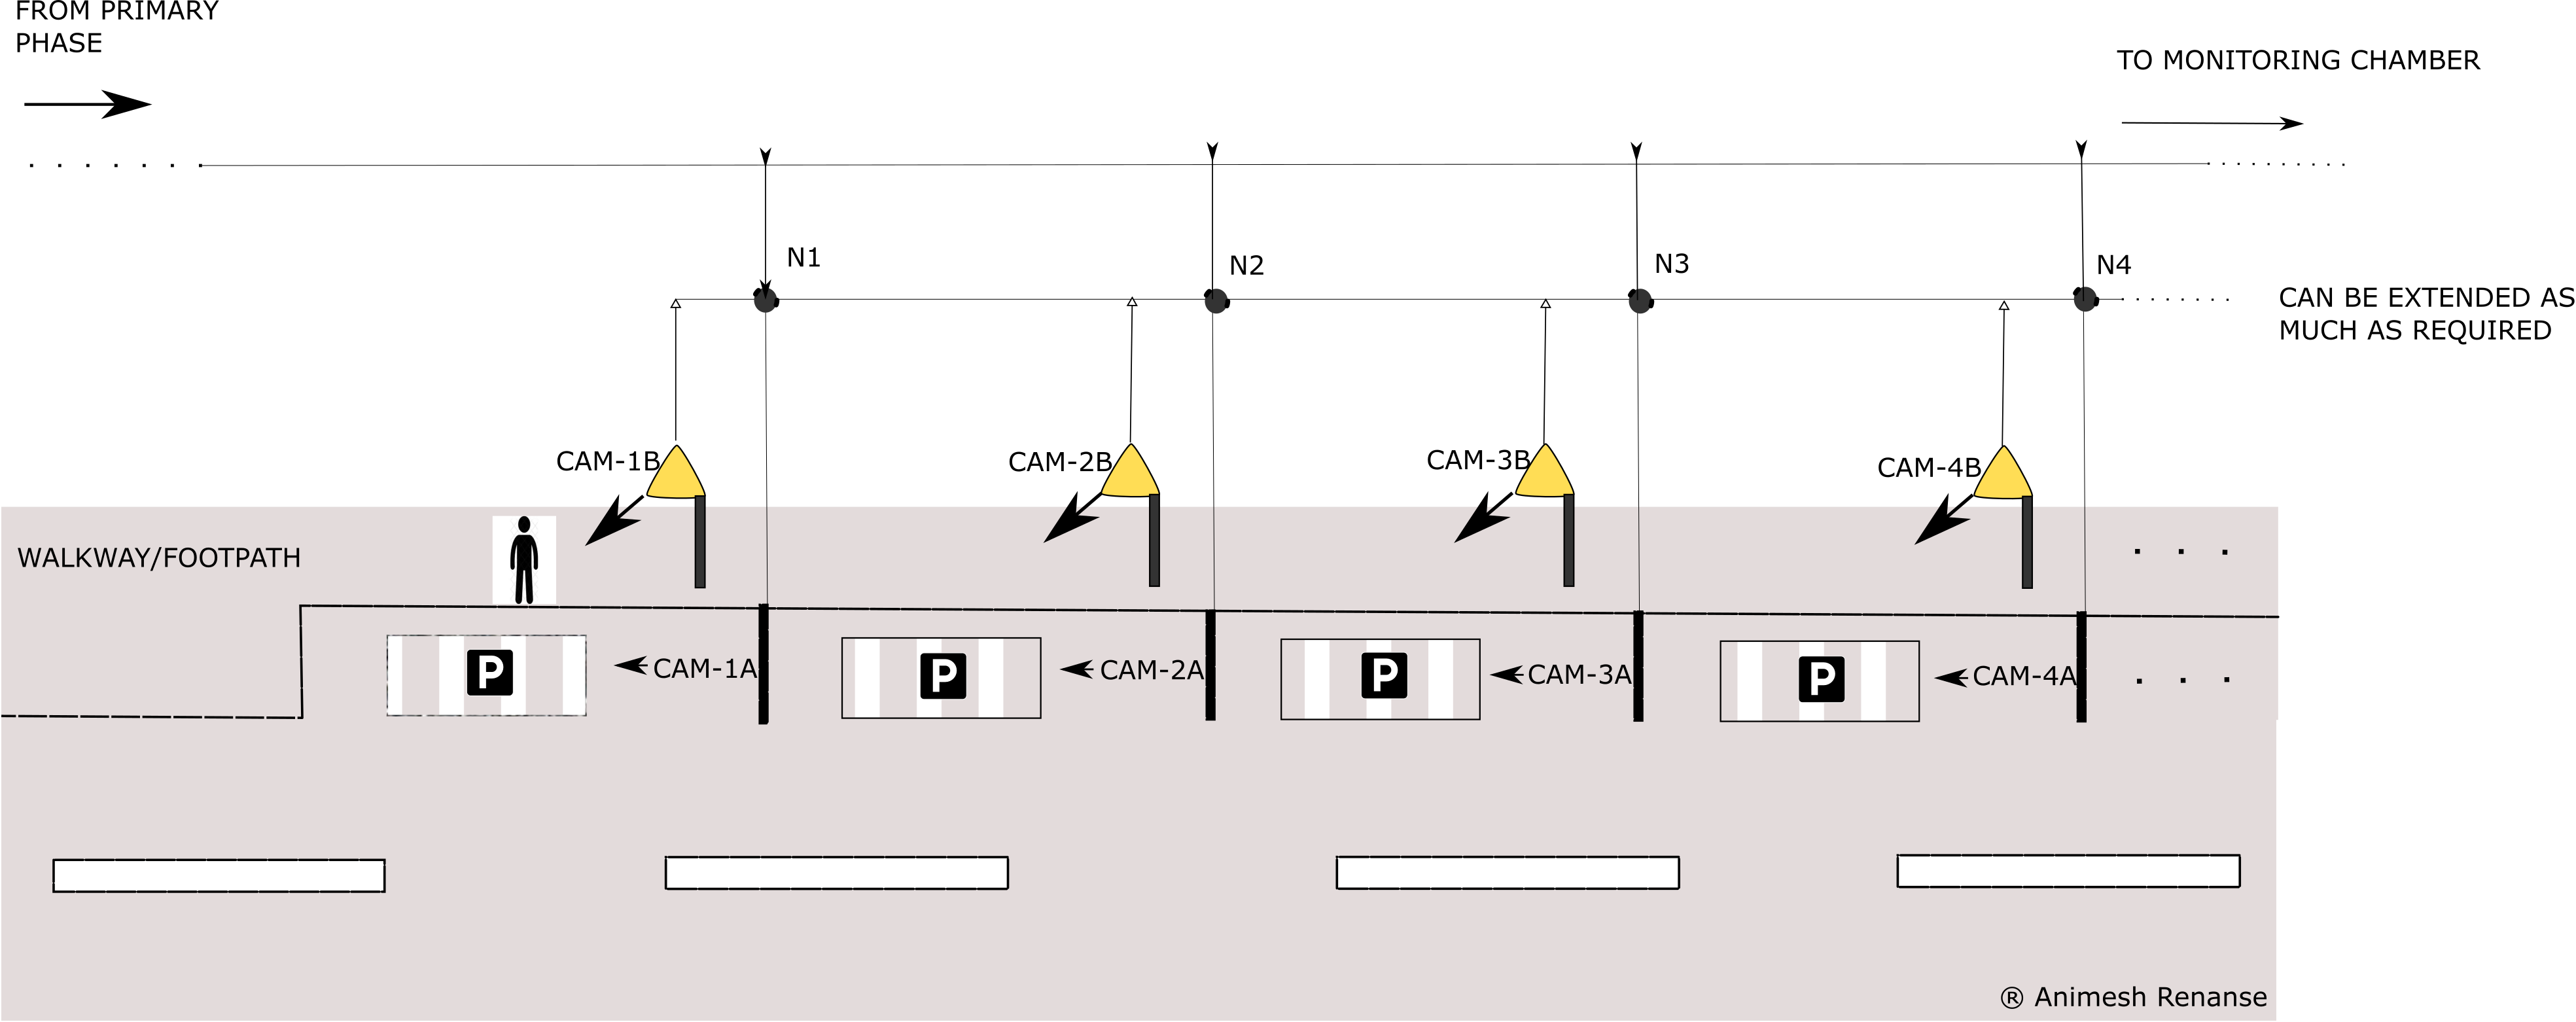
\includegraphics[width=8cm,height = 19cm ]{Secondary Phase.png}
%TODO DIAGRAM OF GAMMA_2 PHASE AND TECHNICAL DETAILS
\subsubsection{In-Depth: The $\gamma_2$ Phase}
This is the phase where the output of the $\gamma_1$ Phase (i.e. A Threat score) comes in and keeps track of those samples which are above a particular tolerance level in the $\gamma_1$ score.\newline
\newline
At This point, the particular vehicle is already inside the perimeter of the location and thus it stops at the \textit{Drop-Off point}, where the passenger leaves the vehicle after diverting from the main road towards one of the \textit{Parking cum Drop-off Zone}, at which point, two cameras installed at each such parking location turn on and the CAM-(i)A, where A $\in \{1,2,3,4.....\}$ activates to record the number plate of the parked car. \textbf{\cite{LP camera}}
\newline\newline
At this point,if the $\gamma_1$ Threat Score of the current sample was above the Threshold or the SG1 at $\gamma_1$ Phase deemed the current sample to be \textit{extraordinarily suspicious}, then the stored data of the car's License Number , Total Passengers and Front passengers' Facial Sentiment along with their Facial Data are transmitted towards this (i.e. $\gamma_2$) Phase and thus CAM-(i)A records the current sample's License Number, thus in-turn, uniquely identifying the vehicle at $\gamma_1$ Phase which was deemed a \textit{Threat} by the Aggregation of Machine \& Human inputs at $\gamma_1$ phase, thus, taking Threat identification to the next step, i.e. Actual Threat Detection.
\newline\newline
At this point, the passengers of the vehicle is supposed to come down to the Walkway/Footpath provided at the side of the road where the particular person or group of persons, who is, at this point is identified as a Threat (whether it's %%%UPDATE THIS PART ACCORDING TO LEVEL OF THREAT NOMENCLATURE%%%%% 
High level threat or Low level threat, this step will take place) is/are identified by CAM-(i)B where B $\in \{1,2,3,4.....\}$ by Cutting Edge Face Detection Machine Learning Algorithms \textbf{\cite{FaceFirst Platform}} which will remember the Facial Structure at that point which will be used for Face Detection for further analysis of the threat together with the Emotion based Sentiment Reasoner for that instance as by the basic human psychology, if the person have bad intentions, hopefully that will be portrayed through his/her face too, which will also add \textbf{algo to calc it} up to the final Threat level which will be most readily available to the Security Command of the Current Institution, among all the intermediate scores on-demand.\newline\newline
Thus, by now, the possible Detected Threat is just at the outside of the Inner Perimeter and due to this Methodology, we have already detected his/her vehicle's License Plate, Potential Weight of the vehicle, Total passengers in the vehicle and most importantly, the Facial Structure of the person/ group of persons. \newline
Thus, now they can be interrogated or can be checked by the Security Personnel who would've been informed by the Security command of the level of threat, location and Facial and Body Features of the person/ persons, thus reducing the chance of further advancement of the detected threat near the institution and thus preventing any act of terrorism, and thus ensuring better security.
\newline\newline
\textbf{This proposal can easily be integrated with the already in process of being automated support systems at the Airports which uses Biometric Recognition of individual passenger for better service through A.I. to fully utilize the extent of A.I. that we can avail, which will stretch from Security Systems, which this proposal covered to the already being implemented support systems for Quality Service at Airports and other Locations of mass Gathering \textbf{\cite{AI Already}}}
\subsection{Threat Labelling \& Processing}
We will first focus on the choices that'll be provided to the SG1 to identify the current samples' level of threat. SG1 will be provided 4 levels to recognize the threat, given as below:-
\begin{enumerate}
\item{NO THREAT: Default case, should be most commonly used, BASE SCORE: 0}
\item{MILD DISCOMFORT: If SG1 feels that the sample is hideous or \textit{can be a} threat, BASE SCORE: 10}
\item{SUSPICIOUS: If SG1 feels something is wrong with the current sample and will definitely need a check, , BASE SCORE: 45}
\item{HIGH DANGER: If SG1 has a visual clue of clear \& immediate danger, BASE SCORE: 85}
\end{enumerate}
At the levels 3 \& 4, it's assumed that SG1 stops the vehicle (via BOOM BARRIER 1) and proceeds for further confrontation.\newline
\textbf{Due to extreme shortage of space, I'll be skipping the Process how I derived the \underline{Weighing Threat equations} mentioned below.}
\newline\newline
Now, the Threat Weights from the Luggage weight will be given by following equation:-\newline\newline
\[   
Cost_w(a,b) = 
     \begin{cases}
       \text{$\frac{35}{e - 1}(\exp(\frac{2\text{W}_{Lugg}}{\text{W}_{LT}}) - 1)$,}&\quad\text{if $\text{W}_{Lugg} < \text{W}_{LT}$}\\
       \text{$\frac{-65}{1-e^3}\exp(3\frac{\text{W}_{Lugg}}{\text{W}_{LT}} - 3) + \frac{100 - 35e^3}{1-e^3}$,} &\quad\text{if $2\text{W}_{LT} > \text{W}_{Lugg} > \text{W}_{LT}$}\\
       \text{100,} &\quad\text{if $\text{W}_{Lugg} > 2\text{W}_{LT}$}\\
     \end{cases}
\]
where, $\text{W}_{LT}$ is the threshold weight of Luggage allowed, which is:-\newline
$\text{W}_{LT} = 32n_1 + 32n_2 + 12n_3$, where $n_1, n_2$ \& $n_3$ are same as before.
\newpage
\section{Benefits, Limitations, Costs \& Associated Risks}
\begin{itemize}
\item{This proposal, even though being quite ambitious, can drastically reduce the chances of a big event of terrorism in the future and also can reduce the time taken to react to a given threat by many folds.}
\item{Since security is the major priority of many government, private institutions, this proposal can easily fulfill their doubts about the security of their institution, if applied correctly.}
\item{It's not hard to see that this proposal can be most fruitful to the Airport Industry where security is the major concern globally, as this proposal, while improves security by many folds, can also be incorporated with existing and in the implementation phase of many other A.I. based Guidance and Biometric Verification systems which are helping the commuters to pave their wave through large airports and their security. \textbf{This incorporated with our system can easily span the whole spectrum of human needs, from \textit{Security to Comfort and Ease of Guidance}, thus ensuring better customer feedback and satisfaction.}}
\item{The limitations of this proposal arise from the same thing that started it, that is, a digital solution, since all digital solutions require high processing and raw power, it is quite essential to ensure that the power through these systems is maintained at a uniform rate.}
\item{This is where \textbf{Jindal Power Ltd.} can shine and propose an affordable Power \& Systems solution alongside this proposal, thus being \textbf{extremely beneficial for Jindal Steel \& Power Ltd.}}
\item{Other Limitation arises from the fact the fact that these servers need to be monitored and kept track of that there is nothing wrong with all the monitoring systems, which will require some additional human resources.}
\item{One of the major risk, actually engraved in digital security solutions is that of the case where a major blackout and breakout happens, i.e. due to loss of power to these systems or a major malfunction caused by other elements. We can always ensure that there should be a backup power to these at all times but still, that can be damaged, this is actually the major risk of this proposal.}
\item{The total cost of the whole proposal, if we use the hardware and services introduced in the Reference, will be: }
\begin{itemize}
\item{Weighing Platform: \rupee 60,000 to 70,000 can be negotiated.}
\item{License Plate Capture Cameras: \rupee 1,41,017/piece at max, as it can be negotiated to much lower rate.}
\item{Surveillance Cameras: \rupee 38,200/piece at max, but can negotiated to much lower rate.}
\item{Surveillance Face Recognition Platform: \rupee 4,00,000 to 5,00,000 and can be negotiated.}
\item{Boom Barrier: \rupee 70,000 can be negotiated.}
\item{Additional cost for Building Poles and outposts, connections etc., \textbf{this is where JSW group can prosper again in this proposal for providing cement and construction material and labors, thus benefiting JSW group in the process.}}
\item{TOTAL: \rupee 7,09,217 + \rupee1,79,217 per parking spot in $\gamma_2$ Phase at maximum, \textbf{but this can easily be reduced if the manufacturing of these hardware is distributed to JSW group, which in-turn will generate profit for JSW group.}}
\end{itemize}
\end{itemize}
\newpage
\begin{thebibliography}{9}
\bibitem{Weighing Platform}
\textit{\href{http://www.essaedig.com/weigh-in-motion.php}{Click Here for an example of the Weighing Platform Proposed to be used.}}\newline
A Weighing Platform measures the weight of the vehicle over it. The product given here does this in two cycles, one, where it measures the weight of the front axle of the vehicle and the next when it measures the weight of the rear axle of the vehicle when the vehicle completely crosses the platform. The Algorithm that we deploy to approximately find the weight of the luggage is given in the section above.

\bibitem{LP camera}
\textit{\href{https://www.cctvcamerapros.com/License-Plate-Capture-Camera-p/vivotek-ip9165-lpc-kit.htm}{Click here for the LPC camera proposed to be used}}\newline This camera will recognize the vehicle in question by the License Plate of the vehicle and will keep it in memory if the sample seems to be a threat.

\bibitem{FaceRecogCam}
\textit{\href{https://ivcco.com/product/mz-hd32-10/}{Click here for the Surveillance Camera proposed to be used}}\newline
Since this camera is used only to capture the Faces of the Front Passengers and software does the rest of the job, thus this camera is constrained only to produce good quality image for the software to work perfectly. Other cameras can also be used instead of the proposed one as the customer desires.

\bibitem{FaceFirst Platform}
\textit{\href{https://www.facefirst.com/solutions/surveillance-face-recognition/}{Click here for an example of Surveillance Face Recognition Platform proposed to be used}}\newline A Surveillance Face Recognition Platform like one mentioned above will be used to enforce all the above methodologies and their interface with the Hardware. Since the platform here also provide SDK for their product, thus we can customize it according to our needs to employ custom algorithms for Age, Face, Emotion Detection of the person in the picture. Else, we can use other highly customizable toolkits like \href{https://security.panasonic.com/solutions_application/application_solutions/facial_recognition/}{Panasonic Security Solutions} or \href{https://www.nec.com/en/global/solutions/safety/face_recognition/NeoFaceWatch.html}{NeoFace Watch by  NEC Global} as per the customers' request.

\bibitem{Boom Barrier}
\textit{\href{https://www.shop.toshiautomation.com/product/detail/auto-boom-barrier-4-meter?gclid=Cj0KCQjwoKzsBRC5ARIsAITcwXFyCGsABUKta0HFSZRqa32vFrCnRop7TgHqRWi4hC4mPTXo-3gFVKwaArkiEALw_wcB}{Click here for an example of a Boom Barrier}}\newline Since Boom Barrier in our case will be activated only for certain elements (Those who propose some considerable threat) thus, our Boom Barrier needs to be Manual, which, the above link showcases one of the best in class boom barriers. Other types or indigenous manufacturers can be used as per the demand and the process ahead.

\bibitem{AI Already}
Bhumika Khatri, \textit{\href{https://inc42.com/buzz/delhi-airport-to-enable-facial-recognition-tech-under-digiyatra/}{Delhi Airport Begins Facial Recognition Tech Trials For Domestic Vistara Flyers}}. Inc42, $24^{th}$ September 2019.
\end{thebibliography}
\end{document}